\documentclass[a4paper]{article}
\usepackage{amsmath}
\usepackage{amssymb}
\usepackage{parskip}
\usepackage[english]{babel}
\usepackage{ccicons}
\usepackage[margin=2cm]{geometry}
\usepackage{graphicx}
\title{Virtual and Augmented Reality}
\author{Kevin Michael Frick}
\begin{document}
\maketitle

\section{Reality and Models}

Models are necessary to get from question/queries to expected answers,
the correctness of which depends on the complexity of the models

The evolution of models has gone from physical objects to analogue and
then digital models

A model is a simplified representation of reality that reproduces, in
lab scale, the behaviour of a physical system, to allow to study
and design systems that would be too difficult to experiment on

A model can be acquired from an existing object, or created to
allow us to see a non-existent or damaged object

In model acquisition, the data are object points obtained by sensors,
which are digitalized.
It's a semi-automatic process of ``photography''.

Acquisition requires access to the object (fieldwork) and sometimes
gives an incomplete model which, however, is measurable w.
r.
t.
reality

In modelling of non-existent objects, the data are maps, sketches or text
produced by an expert which are e.g. modelled in 3D.
It's a manual
process of ``repainting''.
Modeling can be applied to nonexistent
objects, in order to e.
g.
~compare different historical hypotheses, and
the model is often complete although not measurable w.
r.
t.
reality

\section{Virtual reality}

``The Virtual Reality is the computer interactive simulation from the
point of view of the participant, in which the sensory information
he/she perceives is substituted or augmented.
''

A virtual reality system provides interactive simulation, implicit
interaction and immersion.
Examples of VR systems are head-mounted
displays, VR tables, powerwalls, CAVEs.

VR systems can be immersive or semi-immersive.

VR has applications in medicine, architecture, industrial engineering,
entertainment, cultural heritage.

Interactive visualization means reproducing a virtual world which only
exists as a digital model.
Compared with animation, which is passive and
whose response is previously decided, interactive simulation can
improvise and provide a real time response.
Interactive simulation is
carried out by a three-dimensional geometric representation and the use
of realistic visualization and memory management algorithms,
multiresolution models, visibility pre-processing and the implementation
of ``zoom'' capacity.

Implicit interaction means the system infers what the user wants from
his or her natural movements, i.
e.
~gestures and head movements instead
of interaction with a device such as a mouse.
Interaction and selection
are carried out via naturalmovements, the devices and ocmputer are
transparent, and the user perceives direct interaction with objects
instead of having a ``window to the model''.

Immersion means disconnecting senses from the real world and connecting
them to the virtual environment.
Visual immersion means objects should
exist independently of the visualization device and the notion of
``presence'', feeling of being ``into the space'' should be provided
through stereoscopic vision.
Further immersion concerns acoustics,
touch, smell, taste, and movement (i.
e.
~acceleration).

An example usage of VR is virtual prototyping.
In order to avoid having
to make a physical prototype every timethe requirements are given to
designers and technicians which use a CAD systems to draw a model and a
virtual prototype, which can be evaluated by the client instead of a
physical one.

VR revolutionized the field of human-computer interaction and has
applicatons in industry, medicine, architecture, education, art.

The factors involved in interactive visualization are the levels of
simulation (empirics, cinematics, dynamics, deformations, collisions,
realism of e.
g.
~vehicles and physical systems) and interactivity.

Those involved in implicit interaction are limb position recognition,
voice recognition, gesture recognition and ability to provide virtual
menus.

Finally, immersion involves quality of stimuli, uptade frequency,
latency, cohereng among stimuli and temporal coherence.
An interactive
application with stereoscopic vision and tracking device, as well as a
game for a three-dimensional television using a Kinect as an input
device, can be considered VR applications.
This is because they both
provide three-dimensional immersion by substituting the visual
information coming from the natural world with the ones provided through
stereoscopic vision, as well as a way to implicitly interact with the
environment by performing natural body movements that are tracked by the
Kinect or other devices.

A non-interactive three-dimensional movie or video game, however
realistic, are clearly immersive experiences which however do not
entirely substitute or augment the sensory information the user is
receiving.
In the case of the game, controls have to be given explicitly
by interacting with a mouse and keyboard, and there is no substitution
of the visual experience as the images are displayed on a screen that is
clealy separate from the natural world.
The case of the 3D animation
movie is more complex, since the three-dimensional avatars could, in
principle, effectively replace real images.
However, the user is wholly
aware that he or she is watching a movie, which provides no interaction
and is therefore not as immersive as a virtual reality should be.

\section{Virtual reality devices}

VR systems use specific hardware which comprises a big part of the cost
of a VR system and strongly influences its success.

Other than the five classical senses (sight/vision, hearing/audition,
touch/mechanoreception, taste/gustation, smell/olfaction) there are
other human senses that must be taken into account, such as
equilibrioception / vestibular sense of balance and acceleration,
proprioception / kinesthetic sense of where the various parts of the
body are located, and oyher internals enses like thermoception, pain,
hunger, thirst and so on.

Field of view is the amount of visual angle that can be seen
simultaneously on a display.
The human FOV is around 200 degrees
horizontally, while a HMD can usually only display 40-110 degrees.
The
field fo regard is the mount of space surrounding the user in which
visual images can be seen.
A HMD allows for a 360 deg FOR.
Both FOV and
FOR can be measured in hor and ver diections and they impact immersion
end stereo perception.

Resolution can refer to the total number of pixels or to the number of
pixels per area (dpi) or per visual angle (angular resolution).
The
human eye has a resolution of around 30 cycles/degree.

The color depth is the number of different colors that can be seem.
24
bits of color depth allow for 16M colors, 32 bits alow for 4294M.
In
theory, CRT, LCD, PDP and LED screens can have an unlimited number of
color levels while DLP displays are limited by mirror frequency.

Screen geometry depends on the number of screens (from 1 to 6), their
shape (planar, cylindrical or hemispherical) and their location
(L-shaped, tilted and so on).

Light transfer defines how the light gets transferred onto the display
surface, such as front/rear projection or through special optics.

Another possibility is not having a display surface and projecting
directly onto the retina.
Light transfer dictates which 3D UI techniques
can be used.

Refresh rate depends on the device and corresponds to the number of
times the image is refreshed per second.
It corresponds to different
concepts on CRT, LCD, DLP displays.
If the refresh rate is too low, the
image flickers.

Frame rate depends on the application and corresponds to the number of
times a complete frame is drawn on the framebuffer.
Low frame rates
correspond to non-smooth animations.

\section{Visual display systems}

Head-mounted displays (HMD) and head-coupled displays (HCD) are devices
that do not allow for perceiving the outside world and use tracking
sensors to display the image.
HMDs use LCD screens and many of them have
a handicap on FOV, while HCDs use CRT screens and allow for accurate
tracking.

Some examples of HMDs are the HTC Vive and the Oculus Rift.
Both have a
resolution of 2160x1200, a FOV of 110 degrees, an accelerometer and a
gyroscope.
The Rift has a 360-degrees tracking system while the Vive has
a double laser tracking system.
The area of the Oculus is 1.
5x3.
3 while
that of the Vive is 4.
5x4.
5.
A disadvantage of both systems is that
since the pixels are relatively far away, accuracy is lacking in lateral
view.

\section{Projection-based displays}

The Powerwall/CAD-wall was one of the first multi-channel walls.
It uses
an array of projectors.

Workbench/ImmersaDesks can be used as a virtual tabletop, while
holobencehs such as Barco Consul have an L-shaped configuration to le
the virtual object ``protrude'' from the screen.

Curved screens and reality rooms are used in a mono configuration for
various driving, flight and navigation simulators.
A stereo
configuration is less common due to multiple handicaps.

Domes and spherical displays are most often found in aircraft simulation
and planetariums.
It's a challenging configuration due to the
requirement for multi-sided blending and it is not suitable for stereo
since it either provides no added value or causes various parallax
issues.

CAVE systems usually have anywhere between 3 to 6 walls, 4 being the
most common.

Projection-based displays are more ergonomic, since the user does not
have to wear the display on their head, do not isolate from the real
world and do not hinder interaction with other user.
Moreover, there is
usually better peripheral vision, user can see their own body, avoiding
HMD-induced disorientation, and there is no head rotation instability
which causes ``flight simulator sickness''.

Volumetric displays are able to address individual points, called
voxels, inside a given volume, using a very fast projector pointed at a
spinning screen.
The resolution and the color depth is limited, opacity
is lacking, the resulting image is small and, of course, they are not
suitable for direct manipulation.
However, there is no
accommodation/convergence conflict.

When a single display contains stereo images images, separation is
needed.
Separation means providing each eye with its needed image and
rejecting the other, and can be carried out through glasses or
autostereocopic displays.

Autostereoscopic displays require no special glasses to achieve stereo
vision, and work through parallax separation.
The image is split into
odd and even columns and optics ensure each eye only sees one group.

However, the user has to stay in a certain place and not move; if they
do, the image is displayed wrong as shown in the following image.
For
this reason, they are a good fit for TV or handheld game consoles.

\begin{figure}
\centering
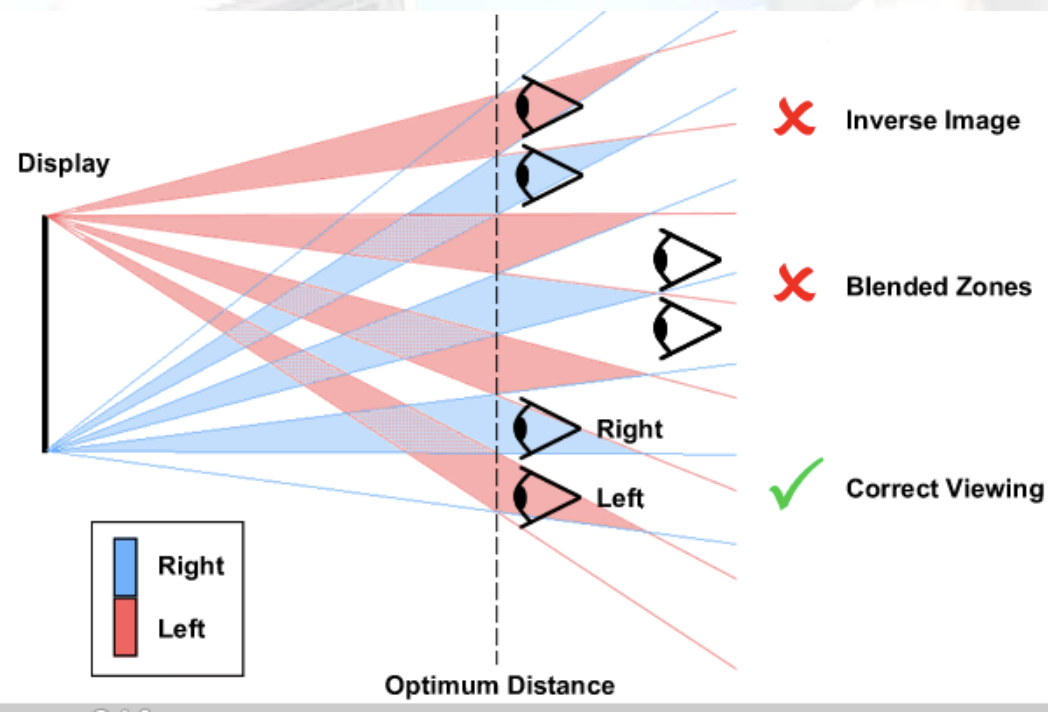
\includegraphics[width=0.75\textwidth]{autostereoscopic-issues}
\end{figure}

Autostereoscopic displays can be implemented with a parallax barrier or
a lenticular array, as shown.

\begin{figure}
\centering
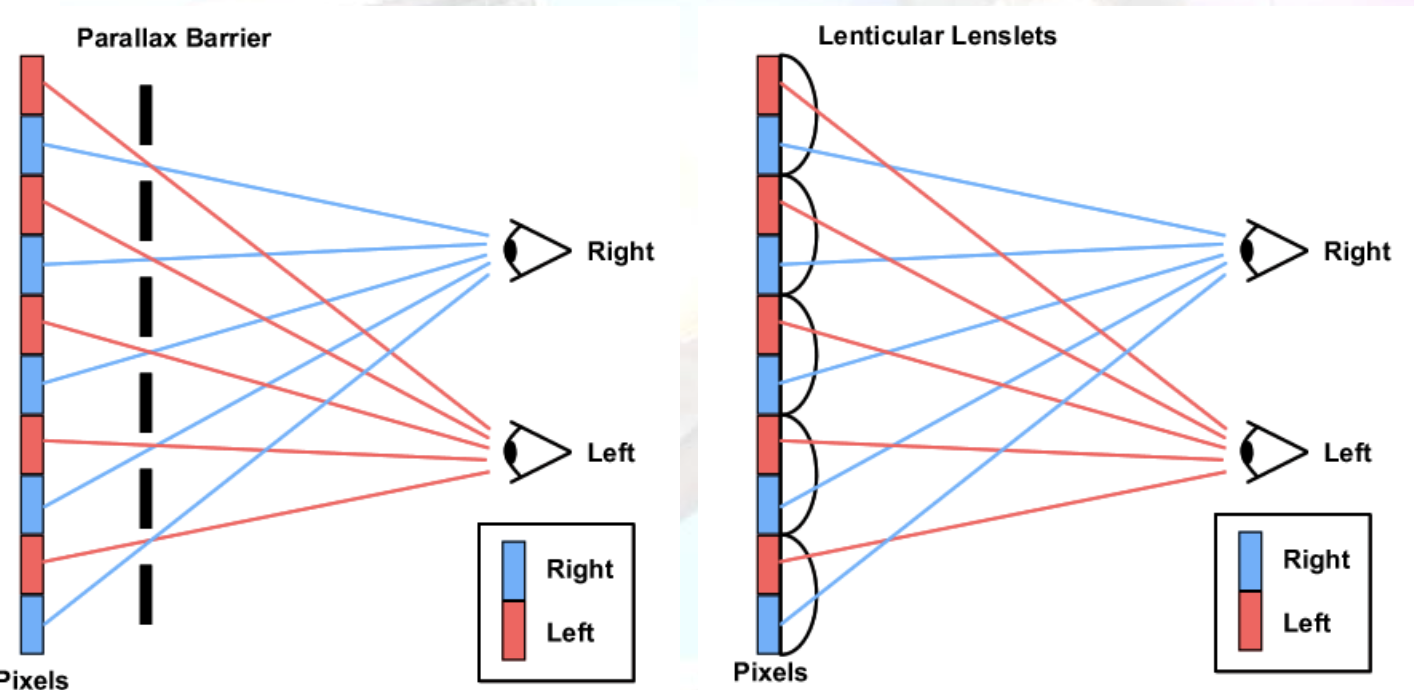
\includegraphics[width=0.75\textwidth]{autostereoscopic-impl}
\end{figure}

Anaglyph glasses are based on complementary colors, e.g. R-GB, G-RB, B-RG.
Each lens blocks two colors and leaves one.
They are cheap, but
have obvious color issues.
Infitec glasses, used for Dolby 3D digital
cinema, are an improved version of anaglyph glasses which ensure each
eye gets red, green and blue light.
Polarizing glasses are based on two
perpendicular linear polarization filters in the projectors and glasses.

They are cheap, but sensible to head tilt.
Circular polarizing classes
build on the same idea, but are almost insensitive to head tilt.
Shutter
glasses block light from one eye or the other in sync with the video
signal.
At any given time, one lens is transparent and another is
opaque.
They require a display running at \textgreater100Hz and
synchronization with the display, e.
g.
~via IR or wired signals.
A
dedicate sync signal can be used for stereo-ready cards, or a
pass-through signal on the VGA connector for non-stereo-ready cards.

\section{Input devices}

Input devices, or sensors, capture the user's actions (e.
g.
~head
movements) and send them to the computer which is in charge of the
interactive simulation.
Input devices are considered VR devices when
they use the paradigm of the implicit interaction or they give 3D input
to the system.

Tracking input systems are sensors which capture the
position/orientation of a real object.
If they only capture position
they have 3 degrees of freedom, if they only capture orientation they
have 2 or 3, and if they capture both they have 6.

Applications of head- and eye-tracking are displaying different images
based on eye position and implementing navigation based on head
movements.

Hand- and device-tracking, on the other hand, allow for direct
manipulation of objects with multiple metaphors, hand-based navigation
together with gloves, and communication with other users using sign
language.

Finally, face- and body- tracking allow for interaction based on the
avatar, e.
g.
~in games, and to capture complex movements offline, which
is useful e.
g.
~in sports.

Position can be calculated absolutely, in known units w.
r.
t.
a fixed
coordinate systems, or relatively, as a displacement w.
r.
t.
an initial
or previous position.
This requires calibration (the initial position
must be known) and is inexact as error tends to accumulate.
When
calculating orientation, two reference frames are defined.
The global RF
is fixed on e.
g.
~the emitter, while the global RF is dynamic and moves
with the object.
The rotation (GT matrix) which transform the global RF
to the local RF can be represented using direction cosines, Euler
angles, angle-axis representation, spherical/polar coordinates or
quaternions.

\section{Technologies for motion capture}

MoCap is the sampling and recording of the motion of things as 3D data.

The first example are Muybridge's sequential photos using multiple
cameras and Marey's single camera and motion capture suit.

MoCap systems can be optical or non-optical.

Magnetic trackers are based on the attenuation of orthogonal magnetic
fields.
Each system includes an emitter, which generates the magnetic
field, receptors which detect it and a control unit.
The emitter is
fixed, defining the global RF, and has three orthogonal coils through
which electric current flows, rotating.
Each coil produces a magnetic
field which is perpendicular to the others.
The sensors are fixed to the
object that has to be followed and have three coils, but the measurement
is the induced electric current by the magnetic field wich surrounds the
sensor.
Usually, the sensors are tied to the control unit by a cable.

The control unit gives power to the emitter, reads data from the sensor
and solves an underdetermined equation systems in 6 (DoF) variables and
9 (3 sensors * 3 fields) equations which results in a hemisphere
equation.
The data is then sent e.
g.
~via RS-232.
Magnetic trackers do
not require LoS, are very precise, and use multiple small sensors.

However, their area of action is limited (2-10 m), they are sensitive to
ferromagnetic surfaces or other magnetic fields, and are wired.

Optical trackers are based on image processing and can be based on
stereo cameras, laser, or other techniques of image processing such as
silhouette tracking.
When using stereo cameras, markers are usually
required, such as color points (passive markers) or LEDs (active
markers).
Optical trackers can register a large amount of points and are
relatively cheap, but have limits in LOS and FOV (given by the camera
FOV), cause overhead or need a dedicated processor, and have variable
latency time.
Optitrack is a particular optical tracker which uses lots
of cameras and IR beamers on the perimeter of the tracking areas, as
well as small reflective balls as markers.
The software will look for
these balls and will extract the 3D position and rotation of objects
from the camera frames.
The tracked objects can be passive because the
cameras have built-in IR lights, it's very accurate and can cover spaces
of any size and shape, but it's very expensive, as much as 50k\$ for a
modest setup.

Acoustic trackers are based on the measure of propagation time (time of
flight) of acoustic signals, usually ultrasounds, generated by
loudspeakers and recorded by microphones, one of which is fixed while
the other is mobile.
When there is a mobile emitter and three fixed
receptors, position can be calculated with 3 DoF as an intersection of
three spheres.
When there are three emitters and three receptors, both
position and orientation can be calculated.
Acoustic trackers are very
cheap, but have LoS issues, latency proportional to the distance, low
precision and are sensitive to ambient noise, echo etc.
which can
distort the signal.

Mechanical trackers are articulated structures with potentiometers
attached to the joints, each of which measures the angle of rotation
w.
r.
t.
a fixed base point.
The position and orientation of the free
parts are a concatenation of translations and rotations.
Mechanical
trackers are very fast and precise, having almost no latency, and are
electronically very simple, but they require to fix the object to the
free part of the structure, limit the freedom of movement and their cost
varies depending on the mechanical structure itself.

Inertial trackers are based on small devices which measure the
acceleration they are experiencing through accelerometers and
gyroscopes, then integrate twice to obtain position.
They have an
unlimited area of action, do not require cables and are not tied to a
fixed reference frame, but the position is relative, the errors
accumulate and the absolute position is not exact.
Moreover they are
sensitive to movement speed.

Data gloves allow to detect the position of the user's finger, expressed
as flexion angles for each finger (3 per finger, 2 for the thumb).
They
are usually combined with trackers.
They allow direct manipulation of
objects, intuitive interaction e.
g.
~with menus, and sign-based
interaction.
Data gloves can be made using optical fiber, by measuring
the attenuation of light which goes through one of two circuits per
finger of optical fiber that has gone through a soecific treatment.
The
attenuation of light, i.
e.
~the difference between emitted and received
light, depends on finger curvature.
Optical fiber gloves are very
precise, fast and ergonomic, but they require constant calibration and
the curvature of the fiber does not always correspond to that of the
finger because of friction.
Mechanical gloves exist that use
potentiometers, similarly to mechanical trackers, or measure the
elongation of a telescopic tube.
Such gloves are exact, precise, fast
and allow for force feedback, but are expensive and non-ergonomic.

Resistance gloves use resistive ink, a special covering whose electrical
resistance is a function of elongation, which is very cheap but not
precise.
Mattel's PowerGlove uses this technology.
Optical gloves,
finally, are based on LEDs or passive markers captured by cameras.
They
have no cables and are very ergonomic, but have LoS issues, high latency
and lack of accuracy.

The Kinect is a low-cost controller made for the Xbox 360 that offers
full-body tracking as well as face and voice recognition.
Its main
components are a color CMOS camera, an IR projector and camera that are
used to measure depth, four microphones, a motor and an accelerometer
for tilt control.
The color camera offers 480p@30fps output while the IR
camera has a 1024p sensor but also only offer 480p@30fps output.
The
operation range is between 0.
4m and 3.
5m, the FOV is (58H, 45V, 70D),
the spatial and depth resolutons at 2m distance are 3mm and 1cm,
respectively.
The IR emitter projects an irregular pattern of IR dots at
varying intensities, and the IR camera reconstructs a depth image by
recognizing the distortion of this pattern.

Examples of other input devices are car simulators, flight simulators,
locomotion interfaces such as omni-directional treadmills whose surface
can move in any direction.

The most modern approaches are all-in-one solutions such as the Vive
Focus Plus, which inegrates a viewer with a resolution of 2880x1600 and
a FOV of 110 degrees with a Snapdragon CPU, 32GB ROM and 4GB RAM, with a
tracking system that does SLAM directly on the HMD via an accelerometer,
a gyroscope and computer vision algorithms.
Moreover, there are two
controllers which have 6 DoF and offer sensor fusion with IMU sensors.

The motion capture pipeline is:

\begin{enumerate}

\item
  Studio setup
\item
  Calibration of capture area
\item
  Movement capture
\item
  Data cleanup
\item
  Data post-processing
\end{enumerate}

\section{Markerless mocap}

Markerless motion capture algorithms analyze input images, identify
human forms and track the optical flow of the scene.
Depth-based mocap
uses a combination of color cameras and depth sensors to capture the
silhouette of the subject from multiple angles and reconstruct the
object's volumetric mesh from thepoint clouds, then fit a skeleton into
the 3D model to estimate motion.
Vision-based mocap, on the other hand,
uses a single or multiple RGB cameras and deep learning, using large
amounts of training motion data.
These examples have been generated
using computer graphics, and the algorithms learn a random forest that
maps depth images to body parts, transformin it into a skeleton.
In
order to improve the skeletons we can use temporal information given by
a tracking algorithm and reject ``bad'' skeletons in favor of ``good''
ones using some ground truth database.

Mocap is faster, cheaper and scales better than frame-by-frame animation
but software and hardware are expensive, capture systems may impose
requirements on the space, and artifacts can occur if the animated model
differs in proportions from the captured model.

The HTC Vive operates following the \emph{inside-out principle}.
There
are no external cameras.
Two laser emitters are used instead, called
Lighthouses, which alternate in sending hor and ver IR laser sweeps
spanning 120 deg in each direction.
The Vive's headset and controllers
are photodiodes and can indicate when the laser hits them.
The time
difference in the hits allows for recovering the position and
orientation of the headset, which are used to integrate the primary
measures (which come from IMU sensors) and correct for error that is
built up over time.

\section{Post-processing in mocap}

Mocap data applied without post-processing introduces artifacts such as
floor intersections, footskating, joint orientation discontinuities.

Retargeting, or ``computer puppetry'', which is re-using motion data
adapting animated motions between characters, suffers from the issue of
differing heights.
The aim is preserving the essence of motion, but the
problem is whether angles or end-effector positions should be preserved.

The issue of motion retargeting is a constrained optimization problem
where a functon \(g()\) of the motion \(m(t)\) has to be optimized while
satisfying a set of constraints, \(f(p) = 0\), in order to adapt to the
target character.
This optimization problem, however, is too costly to
solve directly, therefore an importance-based approach is applied that
uses a heuristic to evaluate importance of joint angles or end-effector
positions.
The problem of computing the angles from end-effector
positions, in order to find the constraints that have to be imposed, is
called inverse kinematics and consists in using the kinematics equations
of an articulated rigid body yo determine the joint parameters that
provide a desired position of the end effector.

Motion planning is the specification of the list of movements that a
humanoid has to carry out in order to achieve a task.
Inverse kinematics
are useful because new motions can be synthesized from a small set of
pre-recorded animations.
This can be combined with physics-based
simulation to create complex motions.

The goal of inverse kinematics is computing the vector of joint DoFs
that will cause the end effector to reach a desired goal state.
Several
solutions (or none) may exist, and the computation is expensive.
Capture
data is voluminous, and capturing all possible motion is implausible.

Data is therefore organized, represented and combined with itself and
with physics simulation in order to dynamically generate new motion.

\section{Stereoscopy}

Stereoscopic vision is one of the most important depth cues, plays a key
role in all VR applications and influences both software and hardware.

Human retinas only planar images, but the human vision system can
recover depth information by combining various depth cues.
While in the
real world, all depth cues agree, some may disagree in VR.
Poor
stereoscopy leads to poor depth information and eye strain, which can
even cause motion sickness if the stimuli are excessively conflicting.

Monocular depth cues only depend on one image, and are:

\begin{itemize}

\item
  Shading, which largely depends on surdace orientation and thus
  provides depth information
\item
  Shadows cast by objects
\item
  Retinal image size
\item
  Linear perspective, that is distant objects appearing smaller and
  parallel likes appearing to meet at a vanishing point at the horizon.

  Depth can be compressed by increasing focal length or decreasing FOV
\item
  Texture gradient, i.
e.
~the further apart is an object, the higher the
  spatial frequency in its texture
\item
  Atmospheric perspective, i.
e.
~light scattering by the atmosphere (fog)
  that makes farther objects look hazier
\item
  Motion parallax, that is the fact that when the observer moves, the
  retinal images of objects close to the eye are displaced more quickly
  - and through a larger angle - than are the retinal images of more
  distant objects
\item
  Occlusion/interposition, which is the most important monocular depth
  cue.
Objects that block other objects appear to be closer
\item
  Accommodation, i.
e.
~deformation of the eye lens (cristallino) which
  allows to focus objects at some distance.
The larger the pupil
  size/camera hole, the closer is the focused part of a scene
\end{itemize}

Binocular depth cues depend on the ability of humans to see two images
from the two eyes, and are:

\begin{itemize}
\item
  Convergence which happens when the eyeball rotates, allowing us to
  place the point being fixated on at the fovea, a point of the retina
  which is responsible for sharp central vision.
In other words,
  accommodation is the focusing motion that happens by deforming the
  cristallino, while convergence is the turning inwards motion we feel
  when fixating on a close object.
Normally, there is a natural
  relationship between accommodation and convergence.
However, when
  looking at a screen, the images on the screen are located in different
  places.
As a consequence, the location of the geometric image, seen
  stereoscopically, lies away from the plane of the screen.
As shown in
  the following figure, the eyes accommodate on the screen, but converge
  on the location of the stereoscopic image, causing a conflict known as
  vision decoupling.
The Oculus Rift VR headset's lenses provide
  collimated light, therefore the eyes accommodate at infinity when
  wearing the headset.
This means that the accommodation/convergence
  conflict is going to take place every time the user is looking at
  something that is not infinitely far away.
The same conflict holds in
  the HTC Vive VR headset, where the eyes accommodate on a screen that
  is very close to the eye, but then converge on points whose depth is
  highly variable.
Holographic (spinning mirror) displays can allow a
  single eye to focus on the virtual object in when the viewpoints are
  close enough to approximate a continuous 3D light field wavefront.

  This way, the depth cue of the virtual objects can be captured by the
  accommodation process of human eye, allowing it to accommodate on the
  virtual object and eliminating the accommodation/convergence conflict.

  Auto-stereoscopic displays are a textbook example of a device that
  breaks the accommodation/convergence relationship, since a point that
  is positioned at a different distance from the eyes than the screen is
  using stereoscopy causes the eyes to converge on that point while they
  are accommodating on the screen, thus causing vision decoupling.

\item
  Retinal disparity, the difference in left and right images of an
  object due to the horizontal separation between the two eyes.
The
  ability to combine two images with disparity into a single image with
  depth is called fusion and the resulting sense is called stereopsis.

  The two eyes define a horopter, a surface that for a given convergence
  has no retinal disparity.
Points closer to the eyes than the horopter
  have crossed (negative) disparity, while points farther have uncrossed
  (positive) disparity.
The area around the horopter where binocular
  fusion is possible is called panum, and outside of it fusion fails,
  resulting in double images.
Near the fovea, the maximum binocular
  disparity resulting in fusion corresponds to 1/6 of degree of visual
  angle.
Every scene point has its own retinal disparity, and if we
  change the fixation point, we change disparity
\end{itemize}
    \begin{figure}
      \centering
  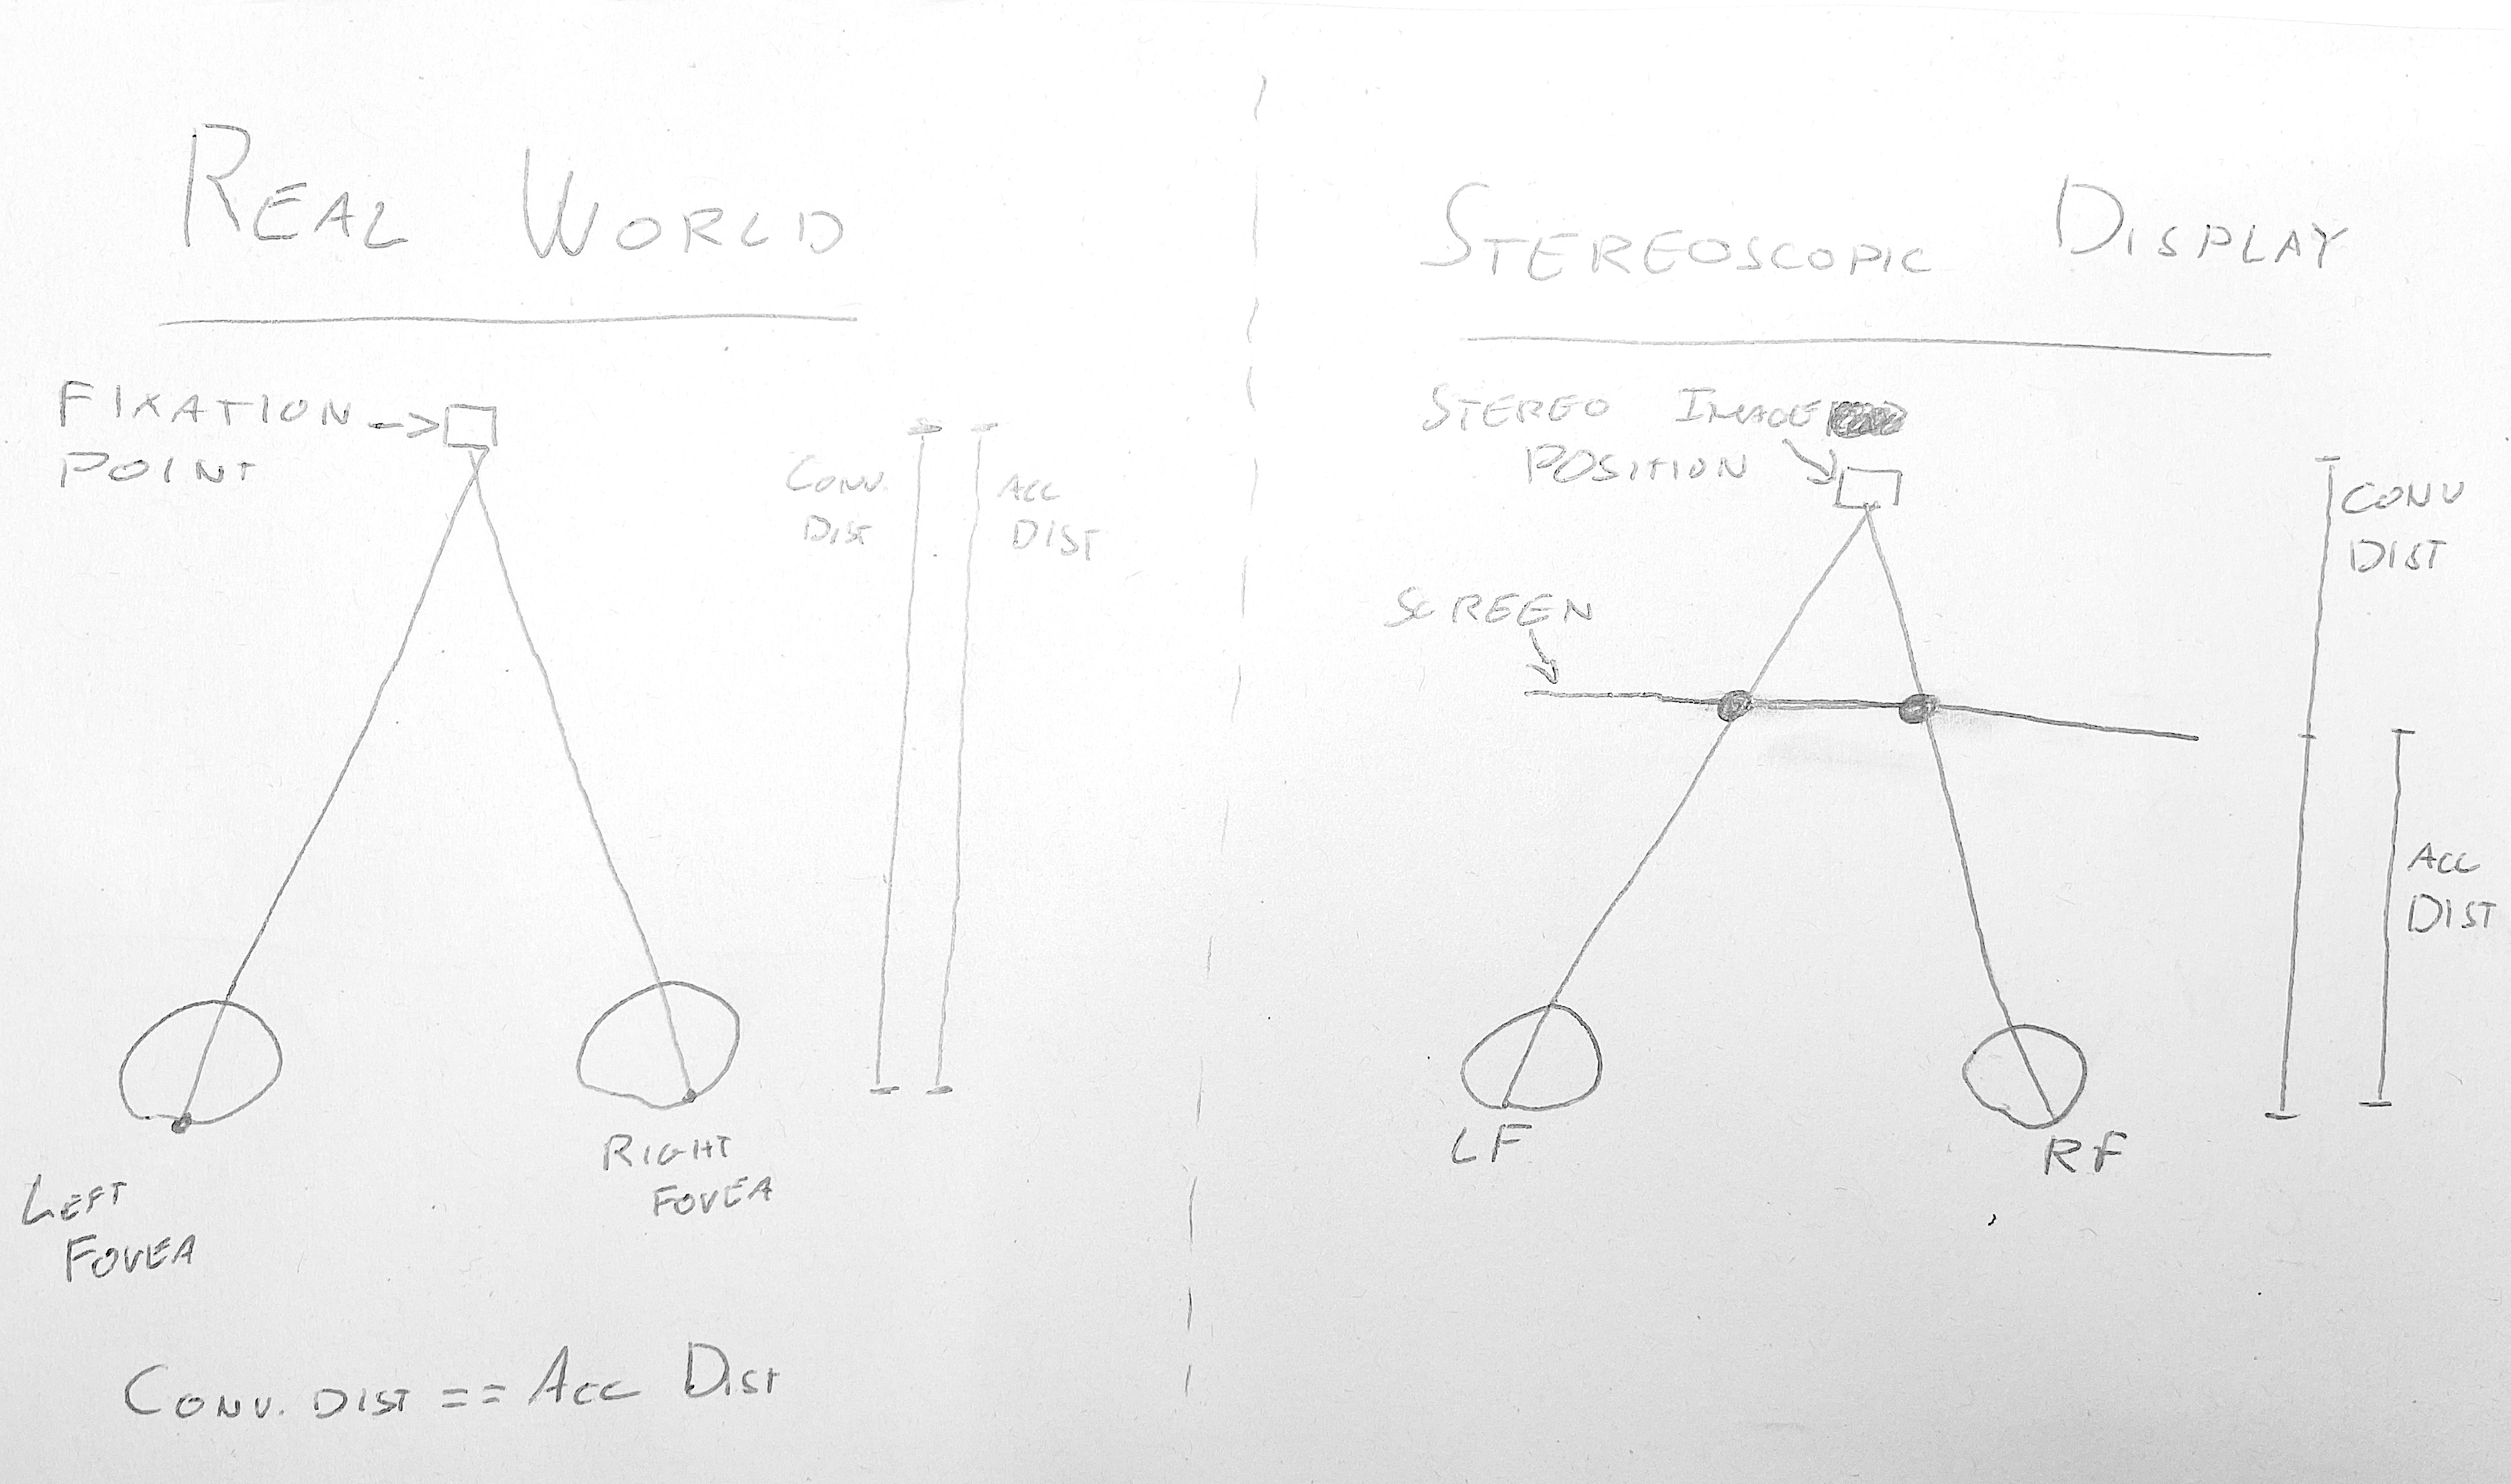
\includegraphics[width=0.75\textwidth]{acc-vs-conv}
    \end{figure}

\section{Stereo camera computation}

The parameter needed are extrinsic, i.
e.
~eye, target and up vector
position, and intrinsic to the camera, i.
e.
~the view frustum geometry.

Stereo rendering is reequire don tiled, multi-screen and head-tracked
displays.

In projection-based systems such as CAVEs and Stereowalls the tracking
data are the L/R eye positions, which can be tracked with two 3DoF
position tracker or one 6DoF data, and the display system data is screen
geometry.
One important parameter for projection-based systems is
parallax.
Parallax is related to, but distinct from, retinal disparity,
and consists in the distance between left and right points as measured
on the screen.
Unlike disparity, parallax does not depend on eye
convergence.
An object has zero parallax wen the corresponding left and
right points overlap, and when looking at it, the eyes converge on the
screen plane, where the object appears to be.
If the left point is to
the left of the right point (positive disance), the eyes converge behind
the screen, where the object appears to be.
If stereo cameras are
computed correctly, parallax is less than or equal to IOD.
Negative
distance corresponds to negative parallax and the object appears to be
in front of the screen plane, where the eyes converge.
Studies recommend
that negative parallax should not exceed 1.
5 degrees, or the object will
be too close.

Fish-tank VR is a low-cost VR system which uses various technologies to
guess the user's location.
One possibility is using a head-mounted
display that follows the head movements, so the screens are fixed w.
r.
t.

the eyes.
The parameters are head orientation, position and the HMD
frustum shape and distortion.

When a single framebuffer has to hold both the left and right images, a
stereo pair has to be encoded in the color buffer.
This does not happen
when there are e.
g.
~two different computers generating each image.

Framebuffers for stereo can be color-based, frame-based, or line- or
column-based.

Color-based framebuffers implement anaglyph stereo via a color mask on
each buffer.

Side-by-side frame-based framebuffers split the screen in two and render
the left and right image on the respective sides.
Quad-buffered
frame-based framebuffers, on the other hand, are used in active stere to
provide both images during the time the application takes to draw the
next frames, which are then swapped simultaneously between the front and
back buffers.
This is only supported by stereo-ready graphics cards and
is a common format when a single monitor or projector is used.

Line- or column-interleaved framebuffers use even and odd line or
columns to encode the left and right images, but in doing this, they
halve vertical or horizontal resolution.

Display generators, finally, convert the content of the front color
buffers into a video signal.
Stereo-ready cards have one video signal
and encode left and right images sequentially; dual-head PCs have two
independent video signals, and there are also quad-head PCs.

\section{Oculus Rift}

The hardware for the Oculus DK2 is composed of a headset and an IR USB
camera for position tracking.
The headset contains head tracker hardware
(IMU), a latency tester, infrared lights, a 1080p display (960 hor px
per eye) and lenses.
The IMU has 6 DoF, 3 for angular velocity and 3 for
linear acceleration; the IR camera also has 6 DoF, 3 for position and 3
for orientation.

The Oculus Rift has an Inertial Measurement Unit (IMU) that reports
angular velocity and linear acceleration.
In order to get position from
acceleration, two numerical integration steps have to be performed as
shown: \[
\mathbf{v} = \int \mathbf{a} dt \implies \mathbf{s} = \int \mathbf{v} dt = \int \int \mathbf{a} dt dt
\]

These two steps magnify the measurement error in acceleration,
eventually leading to position drift.
In order to correct for this
cumulative drift, data from a camera is used, which however has a much
higher latency than the IMU (60 Hz vs 1000 Hz).
For this reason, a
combination of the two sensor is used in order to let the IMU estimate
position via integration and then correct drift when camera position
data is available.

Drift correction is carried out for positon via the tracking camera,
while for rotation, pitch and roll are based on the accelerometer
measuring gravity and yaw on the tracking camera.

Latency is a major issue in VR, with acceptable values being under 20 ms
A sharp turn of 250 deg/s will cause 5 degrees of error with 20ms
latency, which will cause motion sickness.

The FOV for the Rift is around 100 deg hor, 90 deg ver, but the lenses
expand the images so that the perceived FOV is larger.
Eyes are not
centered behind each half of the panel.
The Oculus lenses provide
collimated light, so the eyes accommodate at infinity.
This is good for
presbyopic people and eyes remain in a relaxed focus space.
For a given
point on the display, the angle of light hitting the eye is changed, so
if the HMD is moved w.
r.
t.
the head, in any direction, the part of the
image directly in front doesn't change.

The lenses provide some pincushion distortion, so barrel distortion is
applied in preprocessing in order to provide straight images.
This,
however, also means that more data is presented on the left for the left
eye and on the right for the right eye.

The projection matrices are updated inside a per-eye loop since each eye
can have a different one.
There is a recommended eye order related to
the reresh rate and direction.

The headset runs at 75Hz, providing a 13.
3ms latency, and rendering
should be locked to that refresh rate.
In VR, short-term frame rate
drops are disastrous.
Moreover, the rendering cost is higher because the
entire scene has to be rendered twice, distortion requires more pixels
than eventually displayed, and distortion itself adds some overhead.

Some solutions to aid performance are dynamic framebuffer scaling, which
means rendering to a smaller texture until FPS are high enough, and
timewarp, that is using data from previously rendered frames if the new
one isn't ready at display refresh time, shifting the image to
compensate for the difference between predicted and actual head pose.

Motion sickness is caused by conflicting sensory signals, such as
mismatches between visual and inertial (inner ear) sensations of motion.

The golden rule for VR is that the user is in control of the camera and
that head tracking must exactly match what the user is doing.
When
changing the camera position, the user must be in control of the change.

Default settings such as FOV or scale should not be changed, because
even when ``still'', the eyes are moving a little to compensate for
small head movements (``vestibulo-ocular reflex'').
If the rendered and
perceived FOV are mismatched, those small head movements will no longer
correspond with eye movements and stationary objects will gain motion,
leading to severe motion sickness.

\section{Projection matrix computation}

The position of a point in a given reference frame is given by
left-multiplying the projection matrix (from world space to the desired
reference frame) and the position vector of the point in world space.

For example, we can assume the origin of world space to be in the middle
of the cave, the Z axis pointing downwards, the X axis pointing to the
right wall (looking from the top at the floor) and the Y axis looking in
the opposite direction than the front wall.

The translation matrix \(\mathbf{T}\) is then defined as \[
\mathbf{T} = \begin{pmatrix}
1 & 0 & 0 & F_x \\
0 & 1 & 0 & F_y \\
0 & 0 & 1 & F_z \\
0 & 0 & 0 & 1
\end{pmatrix}
\] with \((F_x, F_y, F_z)\) being the position of the origin of the
reference frame in world space.
At this point, rotation matrices
\(\mathbf{R_x}, \mathbf{R_y}, \mathbf{R_z}\) that encode the rotation
\emph{around} the \(x, y, z\) axes, respectively.
These have the form \[
\mathbf{R_x} = \begin{pmatrix}
1 & 0 & 0 & 0 \\
0 & \cos \theta_x & -\sin \theta_x & 0 \\
0 & \sin \theta_x & \cos \theta_x & 0 \\
0 & 0 & 0 & 1
\end{pmatrix}
\]

\[
\mathbf{R_y} = \begin{pmatrix}
\cos \theta_y & 0 & \sin \theta_y & 0 \\
0 & 1 & 0 & 0 \\
-\sin \theta_y & 0 & \cos \theta_y & 0 \\
0 & 0 & 0 & 1
\end{pmatrix}
\]

\[
\mathbf{R_z} = \begin{pmatrix}
\cos \theta_z & -\sin \theta_z & 0 & 0 \\
\sin\theta_z & \cos \theta_z & 0 & 0 \\
0 & 0 & 1 & 0 \\
0 & 0 & 0 & 1
\end{pmatrix}
\]

Note that:

\begin{itemize}

\item
  the row and column corresponding to the axis of rotation is always the
  unit vector corresponding to that axis (e.
g.
~\((1, 0, 0)\) for the
  \(x\) axis)
\item
  the cosine is always the first to appear when reading the matrix in
  either row-major or column-major order
\item
  a sine and a cosine never appear in the same row or column
\item
  a cosine is never negative
\end{itemize}

Once the translation and rotation matrices have been calculated, the
projection matrix is then defined as
\(\mathbf{P} = \mathbf{T R_x R_y R_z}\).
Note that the translation and
rotation are sensitive to order, so they should be calculated one after
the other, keeping this in mind.

The target is defined by projecting the virtual camera onto the required
screen.

In order to avoid negative parallax, the z-near clipping plane has to
lie on the screen where the projection is being done.

\section{Avatars}

Even in virtual reality, people tend to follow others.
Under stress,
most people won't decide on their own, while with low stress levels they
are more likely to explore the environment.
Therefore, expressive
avatars are needed.

The evaluation of the impact of animations in the perception of a
simulated crowd are both quantitative (velocity, density, flow rates,
personal distances) and qualitative (perceptual evaluation of points,
humanoids, immersion etc.
)

The effect of shape, materia, rendering style, lightness and brightness
affect the perception of facial emotion.
The sense of ``presence'' is
also based on gaze, gait and gestures of avatars.

Experiments show that animation variety increases realism for humanoids
but not for bots.
When using only locomotion, bots' trajectories were
rated as more realistic than those of humanoids.
Appearance alone does
not impact realism significantly.

Minimum requirements for avatars are that height should be adjusted to
the user, animations should be natural looking, and arm movements should
match what is being input through the controller.
When two people are
sharing physical space, they communicate and avoid collision through eye
contact or head movement, while in VR they resort to hand gestures and
verbal confirmations.

Self-location refers to the sensation of being inside a virtual body.
It
is important that in an interactive virtual environment (IVE) the
position of the user's real and virtual bodies match.
Agency refers to
the sensation of having control over the virtual body.
Discrepancies
between what the user sees and what they want to do decreases agency.

Ownership refers to the identification of a virtual body as one's body.

Ownership is related to how ``human'' the virtual body looks, and to
sensory information like visual, tactile and proprioceptive input.

The uncanny valley is the phenomenon where things that look somewhat
human, but are clearly not - such as C-3PO in Star Wars - produce an
accepting reaction, while things that are very nearly human, but just a
little strange - such as a child's doll, a ventriloquist's dummy ora a
clown, - produce a negative response.
The most common criticisms of
characters that fall into the uncanny valley are hollow, lifeless eyes,
waxy skin, poor facial and lip animations.
In order to avoid the uncanny
valley, characters can be either be made empathetic but unrealistic, or
extremely photorealistic through sculpting, texturing and performance
capture.

\section{Human-computer interaction and user
interfaces}

HCI is the process of communication between users and computers.
UIs are
the medium through which the communication takes place, translating user
inputs into a representation the computer can understand and the other
way around.
3D interaction is when the user's tasks are performed in a
3D context; a 3D UI involves 3D interaction.
Affordances and constraints
are what users can and can't do using a technique.

Components of a UI are input and output devices, interaction techniques,
widgets and metaphors.
3D UIs can be more intuitive, can be used to
interact using natural skills, and are more direct, i.e. there is less
cognitive distance between user action and feedback.

User tasks in a virtual environment can be classified as
selection/manipulation, navigation, application control and symbolic
input.

\subsection{Selection and manipulation}

Selection means identifying an object from a set, while manipulation
means positioning, rotating, scaling and deforming objects.
The key
issues in these two tasks are mapping the user action into the desired
results and giving appropriate deedback.

The number of control dimensions is the number of DoFs of the input
device, while the integration of control dimension is the number of
\emph{simultaneous} DoFs.
Ideally there are \textgreater=6 DoFs, fully
integrated.

Isomorphic control is when the device measures the position of the
user's limbs, which is preferable for manipulation, while isometric
control is when the device measures the force applied by the user, which
is preferable for controlling rate.
Isomorphic manipulation where there is one-to-one correspondence between real and virtual hand motions is more
natural and intuitive, but non-isomorphic manipulation overcomes
hardware and human limitations through the use of ``magic'' virtual tools.

There exist hand-attached controllers, such as virtual gloves, and
hand-held controllers, such as VR controllers.
In general, larger
muscles are used for slower movements.

Physical props can be used for selection and manipulation.
In this
context, replicating the shape of the virtual object gives no benefit
for manipulation.

Exocentric metaphors include the world-in-miniature metaphor, in which
the user is provided with a handheld miniature of the scene.
WIM
requires careful use of occlusion management.

Egocentric metaphores include virtual hand and virtual pointers.
When
using a virtual hand, the user selects and manipulates objects directly
with their hands.
Typically, a 3D cursor is displayed and the user
intersects it with the target and uses a trigger technique for
selection, while manipulation is performed through natural hand
movements when the object is attached to the virtual hand.

The main problem is that only objects that the user can reach can be
selected/manipulated, so users are required to travel.

Virtual pointers allow users to select and manipulate objects that are
beyond the immediate reach of their limbs.
It is a very suitable
technique for selection, but manipulation is problematic since only
radial movements can be made, which is bad for changing distance to the
user.
It's also a technique that is only effective for one degree of
freedom, the axis of the pointer itself.
Pointing should therefore be
used for selection, while a virtual hand is better for manipulation.

There are six metaphors for virtual pointers: ray casting, two-handed
pointing, fishing reel, aperture, flashlight and image plane.

When using ray casting, a line segment is attached to the hand and
defines the pointing direction.
This is a very precise technique as the
selection volume is a single ray, but it presents problems in selecting
objects that are far away.
There are many variants: rays can be bent, or
snap to the nearest object etc.
A variant of ray casting is two-handed
pointing, which requires two hands to be tracked in order to allow one
to define the origin and the other to specify where the ray should point
to.

The fishing reel technique is similar to ray casting, but introduces an
additional input device which controls the length of the virtual ray.

Another metaphor is the flashlight, in which the selection volume is a
cone, just like the light in a flashlight.
The apex of the cone is
defined by the position of the user's hand while the axis is its
orientation.
The aperture of the cone is constant.
One issue that is
immediately apparent with this metaphor is deciding which object to
select when the cone comprises multiple objects.
A possible rule is to
select the object that is closest to the axis of the cone, but the issue
still stands when the environment is very cluttered.
A variant of the
flashlight metaphor is using a cone whose axis points to the user's hand
and whose axis is the line passing by the user's hand and eye.
This way,
aperture can be controlled by moving the sensor closer and device twist
can be used to disambiguate between objects.

The fishing reel technique is similar to ray casting, but introduces an
additional input device which controls the length of the virtual ray.

Clutching occurs when a manipulation cannot be achieved in a single
motion, so the object must be released and grasped again.

Each manipulation task has several variables that affect which is the
most suitable technique.
General variables are application goals,
physical and psychological conditions of the users.
The variables involved in positioning are distance and direction to initial and target position, translation distance and required precision.
Those involved in rotation are distance to target, initial and final orientation, rotational distance and required precision.

These task variables should be analyzed when choosing a device, which must match the desired interaction techniques.
Pointing should be used for selection, a virtual hand for manipulation, and degrees of freedom should be reduced when possible.

\subsection{Navigation}

Navigation involves two different tasks, travel (actions to move in the desired direction) and wayfinding (defining a path).

There exist different travel tasks which are defined depending on the user's goal.
Exploration doesn't have an explicit goal and is typically found at the beginning of interaction with a VE.
Search is when the user is looking for some target, and can be naive when the user doesn't know where it is and primer if they do.
Maneuvering involves small and precise movements, e.g. to examine an object, of the head and body.

Exploration is a low-cognitive-load task that allows the user to focus on information gathering and change the target at any moment.
Search techniques can be goal-oriented provided that there is a map with an explicit representation of the target.

There are additional characteristics that should be kept in mind.
Short-range travel can be accomplished by using natural physical motion only, medium-range travel needs some virtual travel technique without speed control, while long-range travel needs speed control and the ability to quickly jump from one point to the other.
Moreover, visibility of the target from the start, DoFs required for the movement (are we walking or flying?), accuracy requirements and the ability to accomplish other tasks are all factors.

In active travel, the user controls the viewpoint, which is controlled by the system in passive travel.
These two types of travel can be mixed in active/passive travel problems such as route planning, where users plan paths that are followed by the system.

Physical travel mimics the real rotational/translational motions of the human body, requiring tracking and being only effective in a limited space.
Virtual travel, on the other hand, happens when the user's body is stationary in a virtual vehicle and only visual motion cues are provided.

One travel metaphor is physical locomotion.

Allowing the user to walk and following their movements provides vestibular cues which help better spatial understanding, but since the VE can't be larger than the real environment - and should usually be smaller, because of physical issues such as cables - it is only suitable for short-range distance.
When users are allowed to both walk and use a virtual travel technique, often they only use virtual travel because it reduces effort.

Walking-in-place, where the feet move but the body remains stationary, solves the need for a large physical environment but is reportedly not effective as real walking.
Users can either be required to just move their feet up and down, or a device such as a treadmill can be used that simulates walking.
Many such devices can cause safety issues if the user loses their balance. Some devices use low-friction surfaces instead of moving parts in order to facilitate locomotion.

A different travel metaphor is steering, that is continuous control of the direction of motion by the user through gaze, pointing, moving the torso, moving a handheld camera, physical steering props or a virtual controller that uses pressure sensors.

Another metaphor is route planning, where a path is drawn by marking points along it, the user being represented by a figure in a WIM o a user icon on a 2D map.

Finally, a last metaphor is map- or WIM- based target specification. Other metaphors include grapping the air, wherein the entire world is an object that can be manipulated, or navigating by reading human thoughts through a brain-computer interface.

Motion sickness comes into play in navigation as well, when a sensory conflict is triggered when a user is moving in VR but not in real life.
Ways to counter motion sickness include teleportation, low speed changes, constraining optical flow to a part of the user's FOV, or using electrical impulses to stimulate the inner ear.

\subsection{Application control}

Informally, application control is defined as the possibility to access the functionalities of an application.
Traditionally, this is carried out in desktop systems through widgets and function keys.

In VR, the application may be requested to perform a particular action, change the mode of interaction or the application state.
Application control is critical because it allows the user to control the interaction flow between selection/manipulation/navigation.
For immersive systems, the traditional 2D GUI elements may or may not be appropriate bacause of differences in DoF, input and output devices.
Factors that influence effectiveness are shape/size/representaton/labeling of the control system, selection methods, potential constraints, and the complexity of the application.

A very simple control method is displaying 2D menus in a 3D world.
Users will instantly recognize them as menus and know how to use them, but they can occlude the environemnt or be hard to find.
Contrary to what may seem intuitive, selection is not that difficult using 3D selection techniques.

When there are only few items, a single-DoF menu can be used, like a ring menu which places items in a circle around the user's hand.
Hand rotation causes the items to rocate, and the selected item is the one within a selection basket.

3D widgets can be colocated, close to the selected objects and used to change geometric parameters, or non-colocated, that is not associated to a particular object.

Menus can be displayed on a separate device, which while allowing to use traditional interaction paradigms is a technique that is only suitable for non-immersive displays and proves quitecumbersome.

Another metaphor is voice recognition, which is a natural and hands-free tecnique but has a high error rate, can disturb other users and requires the user to learn voice commands.
It is a suitable technique for simple commands, but not for e.g. adjusting parameters.

Gesture recognition ofter requires wearing gloves since camera-based recognition suffers from occlusion issues.
The user has to learn gestures as well, so this technique is only useful for a limited set of commands.

The use of familiar devices with real-word correspondences, such as brushes or erasers, allows for physical tool metaphors such as Tangible User Interfaces (TUIs) in which the system draws the virtual representation of a physical tool and the user accesses it by simply picking it up and using it.

Lastly, physical controllers can be used, which are a lightweight way of performing system control which makes it easy to change between modes.
Buttons and switches are not necessarily connected to a menu-like structure and button locations are defined by accessibility / ergonomics rather than functional structure.
A way to indicate functionality is placing a small label or pictogram on the button.

Design guidelines for app control should be:
\begin{itemize}
  \item avoid disturbing the flow of interaction
  \item prevent unnecessary focus changes
  \item avoid mode errors, providing feedback to let the user know the currently active mode, and consider the usage of multimodal input
  \item use an appropriate spatial RF
  \item design for discoverability
\end{itemize}


\section{Presence}

Task performance is an important measure of the effectiveness of a
virtual environment, both within the VE and when transferred outside it.

Another measure of the equality of a VE is presence.

Presence is operationally defined as the successful substitution of real
sensory data by computer-generated sense data.
A ``successful'' response
is realistic, similar to a real response.
Here we are dealing with a
low-level physiological response paving the way for higher-level
cognitive and emotional responses which include verbal confirmations of
``being there''.

Factors that influence presence are display parameters, sound, haptics,
virtual body representation and body engagement.

Presence can be measured with physiological measures, such as heart rate
and galvanic skin response, as well as with behavioral responses.

Subjective methods such as questionnaires are also possible.

Navigating a virtual environment using a controller breaks the
correlation between proprioception and sensory data, while experimental
data confirms this doesn't happen with walking-in-place if the users
associate well with their virtual bodies.

Lower latency also results in a higher heart reate, which correlates
with higher presence.

Visual realism doesn't generally correlate with reported presence.

However, ray tracing makes it possible to have shadows and reflections
inside a virtual environemnt, at the cost of long rendering time.
Real
time ray tracing offes the chance to investigate the impact of dynamic
changes on presence.
Experiments confirm that ray tracing leads to
higher presence than the OpenGL illumination model on the ``pit room''
experiment.

Reported presence is significantly positively correlated with prior VR
experience, but negatively correlated with programming experience and
age.

Presence is used in psychotherapy.
Cognitive-behavioral therapy aims to
restructure patients' beliefs through exposure to feared or traumatic
events.
The patient must experience the anxiety or fear, but not too
much.
VR can help, because the patients know that it's not real but
respond as if it were.
In another experiment concerning fear of public
speaking, people reacted to virtual audiences with appropriate affect,
so it is possible to use VR for treatment.
Of course, when other people
in the VE are real humans, a visual representation of them is needed, to
know what they are looking/pointing at.
Finally, presence in immersive
virtual environments can be used as a validation method for virtual
crowds, to study human behavior under panic or stressful situations that
cannot be evaluated in the real world, and to improve current crowd
simulation models.

Moreover, people wo are in pain from severe burns show alleviated pain
when their consciousness is ``transported to another place''.

Passive haptics are a way of augmenting a high-fidelity visual virtual
environment with low-fidelity physical objects that prevent the virtual
bodies of users from passing through objects.
Passive haptics do not
replicate such properties as texture, thermal conductivity, and mass,
nor do they replicate fine geometric details of the visual objects such
as handles on cabinet drawers.
Examples of static haptics are
head-mounted displays and simple versions of physical objects.

Adding physical objects will improve virtual environments because they
make the objects feel to the user as if the objects are there.
Humans
can test the reality of an image by trying to touch the object, so if
there is a real object where the users expects there to be one, presence
(as measured with heart rate) is increased.

One experiment investigated passive haptics's effects on performance of
a real-world navigation task after training in a virtual environment.

Half of the participants trained on maze navigation in a VE augmented
with a styrofoam physical model, while half trained in a non-augmented
VE but were given visual and audio contact cues.
The task was to gain as
much information as possible about the layout of the environment.

Participants knew before the VE session that their training would be
tested by navigating an identical real maze environment while
blindfolded.

\section{Haptics}
\emph{Tactile} means pertaining to sensory information derived from the skin, \emph{kinesthetic} means pertaining to sensory information derived from limb movement and orientation of body parts, \emph{haptic} is a combination of the two.

A \emph{haptic interface} is a UI that allows a human to have haptic interaction with real or virtual environments.
A \emph{haptic device} is an interaction device actively producing haptic feedback.

The sense of touch is caused when the skin receives a mechanical (mechanoreception), heating (thermoreception), chemical or electrical stimulus.
Pain and ache are caused by nocioreceptors.

\emph{Sensorial accommodation} quantifies the variation in time of the number of electrical discharges generated by a certain receiver in response to a stimulus.
It is usually fast for things that are ``always there'' such as gloves and glasses.

\emph{Spatial resolution} is defined using the \emph{reception field}, that is the are where a stimulus can excite the receiver.
It is positively correlated to the size of the area of the brain that interprets said stimulus.

\emph{Time resolution} is defined as the minimum time to distinguish between two different events.
It is shorter for touch than for sight, and the latter then also needs to be interpreted.

\emph{Proprioception} is the information on the position of the body parts.
\emph{Cinestesia} is the feeling that gives information about the movement of said body parts.
The resolution is measured in degrees and indicates the difference in angle which is not perceived as a change in position.

\emph{Passive touch} is the feeling of an object touching the skin, while \emph{active touch} is produced when touching in active form an object, e.g. pushing a button.
Identification of objects is better with active touch.

Touch is not an absolute sense, and sensitivity is affected by several factors.
Therefore, tactile interfaces should be \emph{scalable} to variability of touch sensitivity.

\emph{Haptic perception} integrates somatosensory information in the recognition of objects.
Touch mediates material properties (e.g. texture, hardness and temperature) and proprioception provides spatial and motor information (e.g. geometry, hand position).

For example, the perceived frequency of grating a finger over a rough surface depends on both the physical frequency and information about how fast the finger is being moved.

In general, visual information is more capable of providing geometric information and a general picture, while touch is more effective in providing material information and fine details.
The ability to correct identify an object is more than double when touch is active, as proved by the cookie-cutter experiment.

Lederman and Klatzky showed that:
\begin{itemize}
    \item lateral motion is effective to discern texture
    \item pressure helps identify hardness
    \item enclosure is useful to size the global shape and volume
    \item static contact allows to feel temperature
    \item unsupported holding is the best way to gauge the weight
    \item contour following is helpful in understanding the shape
\end{itemize}

Vibrating motors entice tactile stimulation by applying motion either directly to the skin or through a mediating structure.
They provide vibration of relatively small amplitude and can be used alone or in arrays.
The most common types are DC motors with an eccentric rotating mass and voice coils.
They are simple, relatively inexpensive, easily powered and controlled and have low power consumption.
However, they do not provide very expressive feedback and vibration can sometimes be irritating.
Finally, it can be hard to miniaturize efficiently.

Linear motors work using pins in an array that are actuated independently and make contact with the surface of the skin.
They are simple and readily available, continuously and rapidly positionable and very versatile, but are very difficult to pack tightly and are relatively expensive because there are several motors per device.

Piezoelectric actuators are single or multilayer ceramic elements which bend when voltage is applied.
Multiple layers amplify this effect.
They can be used to provide very large forces but small motions.
They are small, inexpensive in large volumes, have both high frequency and static modes, have a very fast response time and a low power consumption, but small displacements require accurate amplification and they have a high driving voltage.

Pneumatic systems have three possible output modes based on skin indentation and vibration: suction, air pressure and vortexes.
Using suction draws hair from a suction hole, creating the illusion that the skin is being pushed.
It has a very low spatial resolution and is only appropriate for the palm.
There are two basic patterns of stimulation, large and small holes, and there is a need for lots of equipment to regulate air pressure.
Using air pressure allows for amplitude and frequency modulation to simulate object slippage on the finger, and force feedback on the palm.
Vortexes, finally, can be emitted to an operating distance of about one meter and felt in mid-air using a flexible nozzle that can be controlled to allow for directed sensation.
Pneumatic systems can be more appropriate for some applications and can mimic skin-slip with multiple pockets, as well as allow for mid-air interaction using vortexes.
However, they are not portable, can be noisy, and have difficulties in displaying sharp edges or discontinuities.

The most used contact element is the hand. We need the force range a user can produce and feel and to distinguish between applying a lot of force for a short time or a lower-strength continued force.

\emph{Sensitive bandwidth} is the frequency at which touching stimuli are noticed, and is much higher than the active bandwidth, which is the speed to which it is possible to respond to the stimuli.

\emph{Tactile devices} stimulate the skin to create sensations of contact, \emph{kinesthetic devices} apply forces to influence body movement, and hybrid device attempt to combine the two.

Tactile devices need to have a high stimulation density, their complexity and weigh lower portability, practicality and generality, and finally passive touch does not feel natural and it is difficult to design tactile devices.

Kinesthetic devices have the competing goals of high stiffness and low mass, with force feedback feeling soft and point-based interactions being overly simple.
Moreover, high-quality devices are expensive, and in any case they constrain workspace size and actuation power, usually limiting users to sit at a desk.

Hybrid devices face all of the above challenges, and in addition weight especially is disadvantageous, force and tactile feedback need to be synchronized, there is a tradeoff between complexity and functionality and a need for clever innovation.

\emph{Haptic rendering} is the process of computing and generating forces in response to interactions with virtual objects, based on the position of the device.
Haptic rendering of an object can be seen as pushing the device out of the object whenever it tries to move inside it. The human sense of touch is sensitive enough to require at least 1KHz of frequency in haptic rendering.
To make a surface feel solid, force must be proportional to the depth that is being pushed inside the object.
The frequency of the haptic rendering is much higher than the visual scene graph loop (1000 vs 60 Hz).

The real time surface is parametric, which means that it can be curved to closely match (locally) the real curvature and allows for defining surfaces to define haptic surface effect as a function of position and penetration depth.
Programming APIs use a spherical proxy that stays on the surface of objects and are at the closest point to the haptic device.
3-DoF haptics are limited to applications where poin-object interaction is enough.
6-DoFs are required for applications related to manipulation, such as assembly- and maintenance-oriented design and removeal of parts from complex structures.

There are two types of interaction: point-based haptic interactions have only the end-point of the device (haptic interface point, HIP) interacting with the virtual object through a collision detection algorithm which calculates the depth as a distance between the HIP and the closest surface point; ray-based haptic interactions instead model the probe of the device as a line segment and can touch multiple objects simultaneously when the segment touches them.

In medicine, haptics can be used to model and visualize different tissues without needing to use paid volunteers or dead bodies in training, and are especially useful for minimally invasive procedures.
Finally, applications for carrying out remote surgeries have been developed.

In physical therapy, weak muscles can be supported and trembling can be removed, and assisting forced can be reduced gradually once muscle strength increases.

In sculpting, force feedback can be used for virtual making and later, objects can be 3D printed.

\section{Augmented reality}
Augmented reality is a combination of a real and a virtual scenes.
In augmented reality, the system augments the real world while the user maintains a sense of presence in the real world itself, while in virtual reality, senses are under the control of the system.

In augmented reality, minimal rendering is enough, as well as a small, non-immersive FOV, but high tracking and sensing accuracy is needed.
AR has to keep users from perceiving the difference between the real world and its virtual augmentation.

Most AR applications are focused on enhancing real world activities, and have applications in robotics, manufacturing, hazard detection, archaeology, entertainment, engineering design and consumer design.

AR interfaces have to be be superimposed on the real world, interactive and registered in 3D (appear fixed in space).

Milgram's taxonomy for mixed reality uses three axes: extent of world knowledge (by the computer), extent of presence (by the user) and reproduction fidelity.

An AR display uses optical, electronic and mechanical components to generate images on the optical path between the observer's eyes and the physical object to be augmented.
The display can be retinal, head-mounted, hand-held or spatial optical see-through, or projectors on real objects can be used.

Head-attached devices require users to wear the display systems on their head.
\emph{Retinal displays} use lasers to project images directly on the retina, have a wide FOV, high resolution, brightness and contrast and low power consumption, so they are suitable for mobile or outdoor AR, but existing versions before 2018 were mostly monochromatic and stereoscopic versions were expensive.

Head-mounted displays can be optical or video see-through, whether they let users see the real world directly or through a camera.
Optical see-through HMDs use optical combiners such as half-silvered mirrors or transparent LCDs, while video see-through images combine real images with those from a virtual camera.
They share common limitations of low resolution, limited FOV, a trade-off between ergonomy and image quality, and discomfort due to simulation/motion sickness.
Optical see-through displays suffer from fixed focal length issues, have to be calibrated and are incapable of producting consistent occlusion effects unless incoming light from real objects is selectively blocked.

Head-mounted projective displays (HMPDs) project onto retro-reflective surfaces, while projective head-mounted displays (PHMDs) project onto a diffuse surface.
HMPDs use a mirror beam to redirect the frustum of miniature projectors onto a retroreflective surface located in front of the viewer, phile PHMDs project images onto regular surfaces that the user doesn't "wear".

HMPs decrease the effects of the convergence/accommodation conflict and provide a larger FOV without additional lenses, but offer limited resolution and brightness, which when diffuse surfaces are used depends on the environmental light conditions.

Hand-held device are suitable for wireless and unconstrained mobile handling. Video see-through paradigms are preferred. Hand-held displays in consumer devices have the potential to bring AR to a mass market, but they have limited processing power and screen size, which translates to low FPS and FOV. Moreover, integrated cameras are very limited and these devices do not provide a working environment that is completely hands-free.

However, the \emph{Parks effect} has to be noted. Moving a scene on a fixed display is not the same as moving a display over a stationary scene. In this case, the image persists on the retina and if the display can be moved, a larger image of the scene can be left on the retina.

Hand-held projectors can be used to augment the real environment with context-sensitive content.

Finally, spatial displays detach technology from the user and integrate it into the environment.
There are three different approaches: video and optical see-through and direct augmentation.
Screen-based video see-through make use of video see-through on a regular monitor. They provide a small FOV and limited resolution and are mostly useful for remote viewing. Spatial optical see-through do not support mobile application, have issues with occlusions between real and virtual object and do not allow for direct manipulation, except when using mirror-beam splitters.
In projection-based spatial displays (PBSDs), finally, images are projected directly onto physical objects. There can be a single static or steerable projector or multiple ones.
A stereoscopic projection (and the whole stereoscopy pipeline) is not needed if only surface properties are changed. However, to display 3D graphics, view-dependent stereoscopy is required.
PBSDs are ergonomic, have an unlimited FOV, scalable resolution and no issue with accommodation and convergence, but the user's hands casts shadows, the display is constrained by the looks of the physical object, and projecting onto non-planar surfaces causes blur unless laser projectors are used. Finally, complex geometric and colorimetric calibration is needed.

AR interfaces are classified according to the interaction with virtual objects, on a spectrum between 3D data browsers (with little to no interaction) through 6-DoF devices interaction to tangible user interfaces (TUIs).

When the user cannot interact with virtual objects, the main challenge is only to correctly register them with the real world.
These case scan be combined with a WIM which rotates according to the user's orientation in the real world.

Interaction through 6-DoF devices typically involves selection, manipulation and system control. Typical problems are different input modalities for virtual and real objects and the need to provide tactile feedback.

TUIs use physical objects to interact with the application, which can be tracked by attaching 2D markers used as icons (phicons). In TUIs, both virtual and real objects are manipulated with the hand. An examples are digital desks that register virtual objects only through a work surface and use overhead or back projection to be displayed.

The Microsoft HoloLens can be used for both AR and VR applications. It scans the surrounding environment and displays holograms which interact with it.

The Magic Leap is a retinal HMD which includes an eye tracker.

\section{AR software}

The components of an AR application are libraries for video capture, camera calibration, marker recognition and tracking and object rendering.

AR-Toolkit is a library that searches for markers, finds their 3D position and orientation, identifies them, positions and orients the objects, and renders 3D objects in a video frame. Camera calibration results in finding the camera intrisic parameters.
AR-Toolkit programs consists of an initialization phase where the marker pattern files and camera parameters are read.
Then, a main grab frame - detect markers - camera transform - draw virtual object loop takes place until shutdown.
AR-Toolkit uses three coordinate systems: observed screen, camera coordinates and marker coordinates. Ideal screen coordinates are distorted into the observed screen coordinates.

If the world coordinate system is defined by the marker, there is a different WCS for each of them, and the model matrix would be the identity; othetwise, the WCS is coupled with the camera and the view matrix is the identity.
If at least a marker is stationary, we can set a fixed WCS.
Limitations of AR-Toolkit include weakness to occlusion, motion blur, vignetting, jittering and image noise which can cause false positives and confusion between markers.

Vuforia is a cross-platform library that can track flat image targets, cylindric targets, multiple-image-targets, using frame markers with a binary pattern ID along the border or object markers which recognizes a 3D object using contrast-based features. Vuforia targets are required to be rich in details, have good contrast and no repetitive targets.
Vuforia also allows for creating virtual buttons in the targets, which can be pressed.
Vuforia supports extended tracking, which sustain the tracking when the target is no longer in view using features on the environment.

EasyAR is a cross-platform library that can create and show 3D content using Unity 3D or basic OpenGL and can generate targets at runtime.
EasyAR provides textureless object tracking, illumination-change-resistant tracking, occlusion-resistant tracking, fast and accurate cloud recognition and screen recording.

ARKit is a library for iOS and Unity 3D that uses Visual Inertial Odometry for accurate tracking of the world. Fundamental concepts include world tracking, scene understanding (such as plane detection, hit testing and light estimation), and rendering. It can occlude people, do motion capture and multiple face tracking and work in collaborative sessions.

ARCore is a cross-platform library developed by Google which used Concurrent Odometry and Mapping for accurate device tracking with 6 DoFs. Fundamental concepts are motion tracing, environmental understanding and light estimation.

AR in Unity uses a library called AR Foundation to abstract away ARKit and ARCore and use the proper library for the device that the application is being built for.


\section{AR tracking}
\emph{Registration} is the positioning of virtual objects with respect to the real world.
\emph{Tracking} means continuously locating the user's viewpoint in 6 DoF.
Tracking can be active, passive or hybrid.

\emph{Marker tracking} is a traditional (10+ years) tracking technique for which several open source solutions exist. A rectangle provides 4 corner points which are enough for pose estimation.

\emph{Markerless/natural feature tracking} uses natural cues of real elements (edges, texture, PoIs, lines - used in automated visual servoing) to do model-based or model-free tracking with no visual pollution. Model-based tracking is implemented in OpenTL.

Marker tracking is less demanding and allows for using eye-catching markers, but the environment must be instrumented by markers, which work only when fully in view. Natural feature tracking on the other hand requires a database of keypoints to be stored, but targets might catch less attention, are potentially everywhere and also work if partially occluded.

Outdoor hybrid tracking combines computer vision and inertial gyroscope sensors which both correct for each other. The gyroscope provides frame to frame prediction of camera orientation which is corrected by vision.
Robust outdoor tracking combines hybrid tracking with GPS.

A good AR experience is compelling, intuitive, anchored in the physical world.

Wide area tracking combines panoramas into an offline point cloud model from which camera tracking is initalized and pose is updated by aligning the camera image to the point cloud.

Gesture-based interaction use free-hand gestures to interact, which are captured using a depth camera, and combine gesture and voice input.

Wide FOV see-through displays are composed of an LCD panel combined with a light source on the edge and provide a 110-degree FOV.

It's important to note that a small percentage of adults would be willing to wear AR glasses and many mobile AR browser users experience social issues. This is more of a social than a tecnnical issue.

\section{Advanced rendering for AR}
Virtual objects should seamlessly blend into the real scene to provide a plausible illusion. Light interaction between virtual and real objects should be simulated and the solution should run at interactive frame rates.

To do advanced rendering, the geometry of the real scene has to be known in addition to that of the virtual objects, the bidirectional reflectance distribution functions (BRDFs, i.e. the reflection coefficients and surface normals) should be known, and surrounding illumination is assumed to be distant (coming from a single position).

To capture the geometry, depth cameras are used.
To model the BRDF, we choose a realistic material with known reflection coefficients.

The main ingredients of advanced rendering are instant radiosity, shadow map sbased on simplified geometry, and differential rendering.

The idea of instant radiosity is to use virtual point lights (VPLs) to approximate global illumination
To do so, some directly illuminated points are sampled and are used to provide (reflected) light which are used to illuminate other parts of the scene and handle occlusion.
Shadow maps are then generated for these VPLs by generating depth maps from the points and comparing distances across them to compute occlusion and amount of light received.
This creates a huge performance bottleneck as many VPLs are required for realistic lighting, and even using small depth maps does not alleviate the issue.

To counteract the performance drop caused by instant radiosity, shadow maps generated from simplified geometry (point-based) are used to reduce the number of triangles that needs to be rendered.

First, VPLs are generated only on points that receive direct light from the initial light source. The scene (from the POV of the light source) is rendered onto a cube map, then the amount of light received by each point is computed.
For points that have to have VPLs created, their position and normal vectors are calculated too, which will be the positions and directions of the VPLs.

Second, shadow maps are generated using points instead of polygons. Dual paraboloid maps are used, which provide a compromise between the low distortion of cube maps (which needs 6 cameras) and sphere maps (which only needs 1 camera but has very high distortion).
One paraboloid camera is used, which reflects light at a 45-degree angle.
It has low distortion, can be computed in a single pass, and does not have the tessellation rpoblem when using points.
In a pre-processing step, the algorithm distributes points on the surface and computes the distortion is there is deformation.

Third, notice that depth maps from points have holes (are sparse point clouds).
To do so, the depth image is downscaled performing average pooling ignoring missing data, then the resulting image is repeatedly downscaled and upscaled to fill in missing data.
This method is really fast to implement in real time as well as in parallel, and quality is acceptable.

Lastly, differential rendering is performed to blend virtual objects into the real scene.
The idea is to compute two global illumination solutions and only add the difference to the real scene image.
This minimizes visual error coming from wrong material estimations (which don't match with the real materials) but requires computing two global illuminations in real time.
While computing the real GI, virtual objects are masked in black.
This allows for calculating the influence of virtual objects on the real world and not change the video signal for parts of the image only comprised of real objects.

Any light path can be expressed according to Heckbert in the form (regex) $L(D|S)*E$ where $L$ is a light source, $D$ is a diffuse light bounce, $S$ a specular light bounce, and $E$ is the eye.
To avoid having to render everything twice, we can keep track of the bounces of light paths, and only add them to the ``real image'' if they only cross real objects, or to the ``real+virtual image'' otherwise, taking into account real or virtual blockers. 

\section{Disclaimer}

This document may contain errors and inaccuracies that may damage your
system, cause your partner to leave you, your boss to fire you, your
cats to pee on your furniture and clothing, and global thermonuclear
war.
Proceed with caution.
This document is released under the CC-BY-SA 4.0 license.
\ccbysa
\end{document}
